\documentclass[11pt]{article}


%%%%%%%%%%%%%%%%5
\usepackage[utf8]{inputenc}
\usepackage{polski}
\usepackage{graphicx}
\usepackage{mathtools}
\usepackage{amsmath}
\usepackage{algorithm,algorithmic}
\usepackage[section]{placeins}
\usepackage{titlesec}
\usepackage{interval}
\usepackage[table]{xcolor}
\titlelabel{\thetitle.\quad}



\topmargin=-0.45in
\evensidemargin=0in
\oddsidemargin=0in
\textwidth=6.5in
\textheight=9.0in
\headsep=0.25in

\linespread{1.1} % Line spacing


%%%%%%%%%%%%%%%%%

\date{Wrocław, \today}
\title{\LARGE\textbf{Analiza Numeryczna (M) - Pracownia 1 - Zadanie P1.2}\\Sumowanie liczb zmiennopozycyjnych\\\normalsize{Prowadzący: dr hab. Paweł Woźny}}
\author{Karolina Jeziorska}
        
\begin{document}
\maketitle

\newtheorem{tw}{Twierdzenie}
\newtheorem{alg}{Algorytm}


\thispagestyle{empty}     
\tableofcontents   

\section{Wstęp}
Dodawanie jest podstawym działaniem arytmetycznym. Dlatego chielibyśmy żeby było jak najdokładniejsze i pozbawione błędów - nawet w komputerze. Jednak w arytmetyce zmiennopozycyjnej każde działanie obarczone jest błędem. A czym więcej działań, tym możliwie większy błąd. Dlatego obliczona suma ciagu liczb zmiennopozycyjnych może się znacznie różnić od dokładnego wyniku. Jednak ten błąd nie jest zawsze taki sam - zależy od ilości liczb, ale również od ich wielkości, użytej precyzji czy nawet zastosowanego algorytmu.

Głównym celem niniejszego sprawozdania jest analiza i porównanie różnych metod sumowania liczb zmiennopozycyjnych, aby móc określić, które dają najdokładniejsze wyniki. Przyjrzymy się dokładniej zwykłemu sumowaniu (opisanemu w rozdziale \ref{sec:normal}) oraz algorytmowi sumacyjnemu Kahana (przedstawionemu w rozdziale \ref{sec:kahan}), a następnie przetestujemy oba algorytmy w pojedynczej i podwójnej precyzji (rozdział \ref{sec:testy}).


\section{\textit{Normalne} sumowanie}
\label{sec:normal}
\subsection{Analiza algorytmu}
Naszym celem jest obliczenie $\sum_{i=1}^{n}x_i$ - sumy n liczb rzeczywistych. Można to wykonać za pomocą podstawowego algorytmu poprzez dodawanie kolejnych liczb ciągu $x_i$.
\begin{verbatim}
         s:=0   
         for i from 1 to n
         do
             s:=s+x[i]
         end
\end{verbatim}

\subsection{Analiza poprawności}
Dość łatwo oszacować błąd tego algorytmu

\begin{equation}
\begin{split}
	&\text{Niech } S_{n} = \sum_{i=1}^{n}x_i \text{ i niech } \hat{S_{n}} = fl(\sum_{i=1}^{n}x_i)\\
	&\text{Mamy wtedy: (dla $\delta_1 = 0$)}\\ 	
	&\hat{S_{n}} = fl(x_1 + x_2 + \dots + x_n) =  
	((((x_1(1 + \delta_1) + x_2)(1 + \delta_2) + x_3)(1 + \delta_3) + \dots + x_n)(1 + \delta_n) = \\
	&x_1(1 + \delta_1)(1 + \delta_2)\dots(1+\delta_n) + x_2(1 + \delta_2)\dots(1+\delta_n) + \dots + x_n(1 + \delta_n) \\
	&\text{Gdzie } \delta_i \leq \frac{u}{1-u} \text{ a z ćwiczeń wiemy, że } \prod_{i=1}^{k} (1 + \delta_i) = 1 + \gamma_k \text{ gdzie } \gamma_k \leq \frac{ku}{1-ku} = \theta_k\\
	&\text{Czyli mamy } \hat{S_{n}} = x_1(1 + \gamma_n) + x_2(1+\gamma_{n-1}) + \dots + x_n(1 + \gamma_1) = \sum_{i=1}^{n}x_i(1 + \gamma_{n-i+1})\\
	&\text{Wtedy } |E_n| = |S_n - \hat{S_n}| = |\sum_{i=1}^{n}x_i \gamma_{n-i+1} | \leq \sum_{i=1}^{n}|x_i| \theta_{n-i+1} \leq \theta_n \sum_{i=1}^{n}|x_i|
\end{split}
\end{equation}

Jeśli spojrzymy na pierwsze ograniczenie, zauważymy że zależy od kolejności sumowania - przy pierwszym elemencie sumy kumuluje się największy błąd (można go ograniczyć przez $\frac{nu}{1-nu}$), który przy kolejnych elementach jest coraz mniejszy (finalnie przy ostatnim elemencie można już go tylko ograniczyć przez $\frac{u}{1-u}$). Stąd łatwo wnioskować, że w celu zminimalizowania błędu należy dodawać elementy w kolejności rosnącej, tak by największy błąd stał przy elemencie najmniejszym, a najmniejszy błąd przy największym. Trzeba jednak zwrócić uwagę, że bierzemy moduł z elementu stojącego przy błędzie, to znaczy, że ciąg, który sumujemy należy sortować co do wartości modułu elementów.

Warto również zauważyć, że gdy szacujemy błąd względny, to można go (niezależnie od kolejności sumowania) ograniczyć z góry przez 
\begin{equation*}
	\frac{\theta_ n\sum_{i=1}^{n}|x_i|}{|\sum_{i=1}^{n}x_i|}
\end{equation*}
Jeżeli wszystkie $x_i$ są tego samego znaku - jest to po prostu $\theta_n$. Jednak, jeżeli elementy ciągu są różnych znaków, nie jesteśmy w stanie ograniczyć błędu względnego.



\section{Algorytm sumacyjny Kahana}
\label{sec:kahan}
Algorytm sumacyjny Kahana (nazywany inaczej algorytmem sumowania z poprawkami) pozwala minimalizować błędy, które pojawiają się przy sumowaniu liczb zmiennopozycyjnych w skończonej precyzji. Za twórcę algorytmu uważa się Williama Kahana.
\subsection{Analiza algorytmu}
Algorytm zawiera więcej operacji niż algorytm przedstawiony w rodziale \ref{sec:normal}. Te dodatkowe operacje pozwalają uniknąć utraty mniej znaczacych bitów, gdy dodajemy do liczby względnie do niej mniejszą. Przeanalizujmy algorytm Kahana:
\begin{verbatim}
         suma:=x[1]   
         c:=0
         for i from 2 to n
         do
             y:=c+x[i] 
             t:=suma+y 
             c:=(suma-t)+y
             suma:=t
         end
\end{verbatim}
Zmienna c to poprawka, która zawiera bity utracone podczas dodawania. Na początku wynosi 0, bo suma to dokładnie pierwszy element ciągu. W pętli wartość zmiennej suma może być względnie duża w stosunku do wartości zmiennej y, co powoduje utratę bitów mniej znaczących zmiennej y. W kolejnym kroku operacja (suma-t)+y odzyskuje \textit{zgubione} niższe bity zmiennej y i zapisuje je w zmiennej c, by w kolejnej iteracji utracone bity zmiennej y zostały dodane do następnego elementu ciągu.

\subsection{Analiza poprawności}
Z powodu większej ilości operacji, trudniej jest oszacować błąd algorytmu Kahaha. Wiemy jednak, że:

\begin{equation}
\begin{split}
	&\text{Niech } S_{n} = \sum_{i=1}^{n}x_i \text{ i niech } \hat{S_{n}} = fl(\sum_{i=1}^{n}x_i) \text{ i $\hat{S_{n}}$ zostało wyliczone za pomocą algorytmu Kahana}\\ 
	&\text{Wtedy } \hat{S_{n}} = \sum_{i=1}^{n}(1 + \xi_i)x_i \text{ gdzie } |\xi_i| \leq 2 \cdot 2^{-t} + O(n2^{-2t})\\
\end{split}
\end{equation}

Wykazanie tej zależności przebiega dokładnie tak jak poprzednio, chcemy wyliczyć błąd przy $x_i$. Jednak w tym wypadku łatwiej na to spojrzeć rekurencyjnie - $\hat{s_1} = x_1(1 + \delta_1)$ $\hat{s_l} = (\hat{s_{l-1}} + x_l)(1 + \delta_l)$ (gdzie $\hat{s_l} = fl(\sum_{i=1}^{l} x_i)$), wtedy współczynniki przy $x_1$ to $(1 + \delta_1)(1 + \delta_2)\dots(1 + \delta_n)$, a przy $x_2$ to $(1 + \delta_2)\dots(1 + \delta_n)$ - jak już wiemy, błąd przy $x_1$ jest największy i można nim szacować pozostałe błędy. Wygląda to tak samo w przypadku algorytmu Kahana, jednak współczynnik przy $x_1$ jest trochę bardziej skomplikowany. Spójrzmy więc na wszystkie operacje wykonywane w algorytmie:

\begin{equation}
\begin{split}
	&y_k = (x_{k} + c_{k-1})(1 + \eta_{k})\\
	&s_k = (s_k + y_k)(1 + \alpha_k) \\
	&c_k = ((s_{k-1} - s_{k})(1 + \gamma_k) + y_k)(1 + \beta_k)\\
	&\text{gdzie wszystkie greckie litery są ograniczone przez } u = 2^{-t}\\
	&\text{Chcemy obliczyć wspólczynnik (błąd), który stoi przy $x_1$, w tym celu wyliczamy $S_k$,} \\ 
	&\text{czyli współczynniki przy $x_1$ w $s_k$ gdzie $s_k$ to suma k elementów ciągu.}\\
	&\text{Pomijając obliczenia, które dokładne można znaleźć w \cite{goldberg} mamy}\\
	&S_k = 1 + \eta_1 - \gamma_1 - (4k + 1)u^2 + O(u^3) \\
	&\text{To, co finalnie chcemy, to współczynniki przy $x_1$ w $s_n$, czyli} \\
	&S_n = 1 + 2u + O(nu^2) \\
	&\text{czyli } |\xi_i| \leq 2 \cdot 2^{-t} + O(n2^{-2t})
\end{split}
\end{equation}

Czyli błąd bezwzględny wynosi
\begin{equation}
|E_n| = |S_n - \hat{S_n}| = |\sum_{i=1}^{n}x_i \xi_i| \leq (2 \cdot 2^{-t} + O(n2^{-2t})) \sum_{i=1}^{n}|x_i|
\end{equation}

Dopóki $n2^{-t} \leq 1$ to stała w tym ograniczeniu jest niezależna od n, więc ogólnie ograniczenie jest lepsze niż w zwykłym sumowaniu przedstawionym w rozdziale \ref{sec:normal}. Jednak tak samo jak w zwykłym sumowaniu, błąd względny może być duży, gdy elementy ciągu są różnych znaków (gdy suma modułów jest większa niż moduł sumy).



\section{Testy}
\label{sec:testy}

\subsection{Wyniki}
W celu dokładniejszego sprawdzenia powyższych metod zostały przeprowadzone testy na 3 sumach:
\begin{equation}\label{eq:sum1}
\sum_{k=1}^{10000} k^{-2}
\end{equation}

\begin{equation}\label{eq:sum2}
\sum_{k=1}^{10000} (-1) \cdot k^{-2} + 1
\end{equation}

\begin{equation}\label{eq:sum3}
\sum_{k=1}^{10000} (-1)^{k} \cdot  k^{-2}
\end{equation}

Suma \ref{eq:sum1} to ciąg odwrotności kwadratów kolejnych liczb naturalnych - w przykładzie z zakresu $\interval{1}{10000}$. Jest to więc suma posortowana malejąco, czyli według wcześniejszych rozważań w złej kolejności. Suma \ref{eq:sum2} to liczby przeciwne do odwrotności kwadratów kolejnych liczb naturalnych z dodaną liczbą 1 za każdym razem - wszystkie elementy są nieujemne, ale posortowane rosnąco. Ostatnia suma \ref{eq:sum3} różni się tym od sumy \ref{eq:sum1}, że jest naprzemienna - jej wyrazy nie są posortowane.

Za wyniki dokładne uznaję wartość sumy obliczoną algorytmem Kahana, używając typu BigFloat z precyzją ustawioną na 128 bitów. Wyniki dokładne zostały obcięte bez zaokrąglenia.
  

\begin{table}[!htb]
	\centering
	\begin{tabular}{r|l|l|l|}
	 \multicolumn{1}{c|}{}& $\sum_{k=1}^{10000} k^{-2}$ & $\sum_{k=1}^{10000} (-1) \cdot k^{-2} + 1$ & $\sum_{k=1}^{10000} (-1)^{k} \cdot  k^{-2}$\\
	\rowcolor{lightgray}wynik dokładny & 1.6448340718480597 & 9998.355165928151 & -0.8224670284246132\\ 
	suma normalna 32 & \underline{1.644}7253 & \underline{9998.35}9 & \underline{-0.822467}1\\ 
	suma normalna 64 & \underline{1.6448340718480}652 & \underline{9998.35516592815}8 & \underline{-0.8224670284246}056\\ 
	suma odwrócona 32 & \underline{1.644834} & \underline{9998.3}73 & \underline{-0.822467}\\  
	suma odwrócona 64 & \underline{1.644834071848059}6 & \underline{9998.355165928}226 & \underline{-0.8224670284246132}\\ 
	algorytm Kahana 32 & \underline{1.644834} & \underline{9998.355} & \underline{-0.822467}\\ 
	algorytm Kahana 64 & \underline{1.644834071848059}9 & \underline{9998.355165928151} & \underline{-0.8224670284246132} \\ 
	\end{tabular}
	\caption{\label{tab:wynik}Wyniki sumowania różnymi algorytmami w różnych precyzjach}
\end{table}


Tabela \ref{tab:wynik} pokazuje uzyskane wyniki testów w porównaniu do wyników dokładnych. Podkreślone cyfry to cyfry, które zgadzają się z wynikiem dokładnym, co także pokazują rysunki \ref{fig:wykres1}, \ref{fig:wykres2}, \ref{fig:wykres3}. Można zauważyć rozbieżność dla sumy \ref{eq:sum1} - w tabeli widać, że suma liczona w odwrotnej kolejności (rosnącej) w podwójnej precyzji i algorytm Kahana też w podwójnej precyzji mają tyle samo cyfr dokładnych, natomiast według wykresu wynik policzony algorytmem Kahana ma minimalnie więcej. Związane jest to z zaokrągleniem wartości dokładnej przy liczeniu błędu względnego, przez co wartość dokładna znalazła się bliżej wyniku algorytmu Kahana.

\begin{figure}[!htbp]
  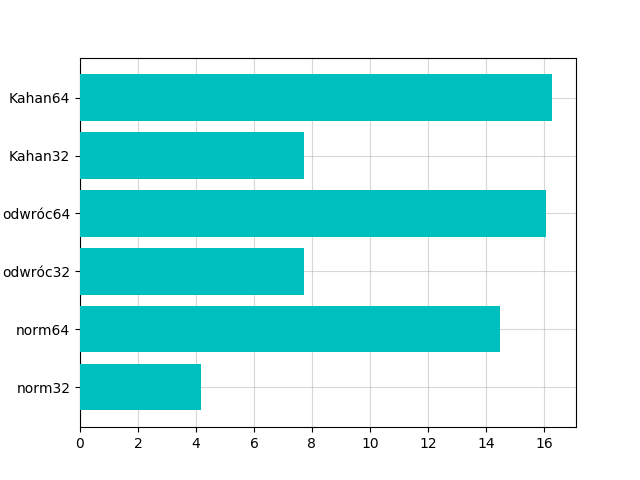
\includegraphics[width=10cm]{figura1.png}
  \centering
  \caption{Liczba cyfr dokładnych dla sumy \ref{eq:sum1}}
  \label{fig:wykres1}
\end{figure}

\begin{figure}[!htbp]
  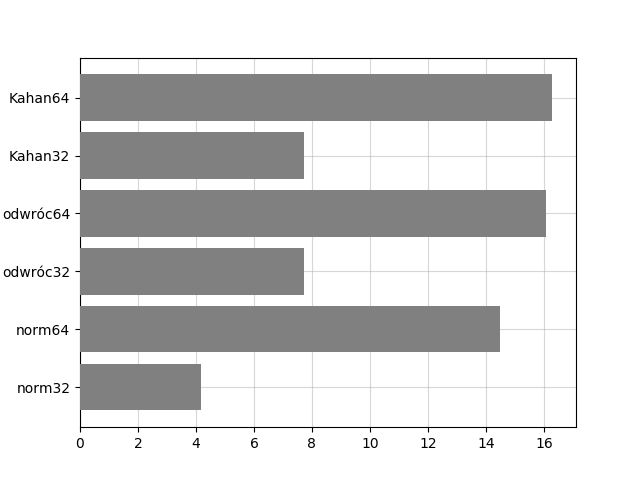
\includegraphics[width=10cm]{figura4.png}
  \centering
  \caption{Liczba cyfr dokładnych dla sumy elementów przeciwnych jak w sumie \ref{eq:sum1}}
  \label{fig:wykres4}
\end{figure}

\begin{figure}[!htbp]
  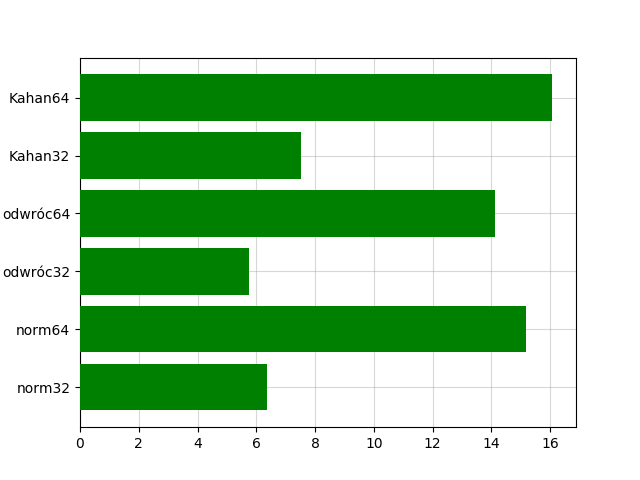
\includegraphics[width=10cm]{figura2.png}
  \centering
  \caption{Liczba cyfr dokładnych dla sumy \ref{eq:sum2}}
  \label{fig:wykres2}
\end{figure}

\begin{figure}[!htbp]
  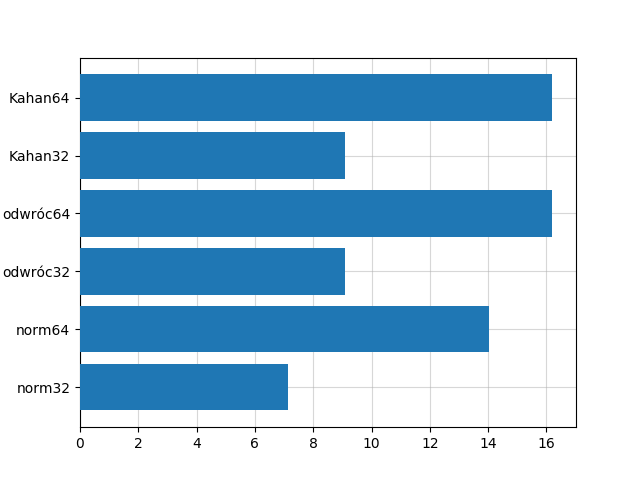
\includegraphics[width=10cm]{figura3.png}
  \centering
  \caption{Liczba cyfr dokładnych dla sumy \ref{eq:sum3}}
  \label{fig:wykres3}
\end{figure}




\newpage
\subsection{Analiza wyników}
Po wynikach testów widać, że przy zwykłym sumowaniu najlepsze wyniki uzyskujemy, gdy dodajemy liczby posortowane rosnąco. Jednak należy sortować  według wartości bezwzględnej liczb, co widać na wykresie \ref{fig:wykres4}, który przedstawia sumę liczb przeciwnych do elementów sumy \ref{eq:sum1}. Wykresy są identyczne, mimo że elementy były posortowane w sposób odwrotny. Ilustruje to zjawisko opisane w rozdziale \ref{sec:normal} - elementy należy sortować co do modułu.


Algorytm Kahana za każdym razem daje tak samo dobre lub lepsze wyniki, niż najlepszy zwykły algorytm sumowania. Patrząc na tabelę (szczególnie na wyniki dla sumy \ref{eq:sum2}), można zauważyć, że algorytm Kahana w pojedynczej precyzji daje tyle samo cyfr dokładnych, co algorytmy normalnego sumowania w podwójnej przecyzji, gdyby wyniki zaokrąglić do takiej samej liczby cyfr dziesiętnych.

Suma \ref{eq:sum3} wydaje się nieposortowana, co jest myśleniem błędnym - jest posortowana malejąco co do modułu, więc wyniki zachowują się zgodnie z oczekiwaniami.
\section{Podsumowanie}
Aby zminimalizować błąd przy sumowaniu liczb zmiennopozycyjnych, można zastosować różne techniki. Najlepszym wyborem jest algorytm Kahana - wykonujemy więcej operacji, ale wynik jest dużo dokładniejszy. Szczególnie jeżeli potrzebujemy wyniku w pojedynczej precyzji.


Jeżeli chcemy ograniczyć liczbę operacji w samym algorytmie dodawania, czyli nie zastosujemy algorytmu Kahana, też mamy możliwość zminimalizować błąd. Trzeba jednak wartości posortować niemalejąco, ale co do modułu. Wynika z tego, że jeśli chcemy policzyć sumę wyrazów ujemnych i dodatnich, należy rozbić sumę na dwie - osobno wyrazów dodatnich i ujemnych (i oczywiście je posortować). Dlatego zwykłe dodawanie opłaca się wykonywać jeżeli mamy już ciąg posortowany (chociaż i tak otrzymujemy potencjalnie gorszy wynik).
\begin{thebibliography}{9}
\bibitem{kincaid} David Kincaid, Ward Cheney
\emph{Analiza Numeryczna},
Warszawa, WNT, 2006.

\bibitem{metody} Germund Dahlquist, Åke Björck 
\emph{Numerical Methods in Scientific Computing, Vol. I},
SIAM, 2008.

\bibitem{higham} Nicholas J. Higham
\emph{The accuracy of floating point summation},
SIAM, 1993.

\bibitem{goldberg} David Goldberg
\emph{What every computer scientist should know about floating-point arithmetic},
Computing Surveys vol.23, 1991.

\end{thebibliography}

\end{document}


